\section{Описание}
В процессе работы использовалось три утилиты, Vlagrind для поиска ошибок работы с памятью, Callgrind для профилирования программы и поиска кода, замедляющего программу и QCachegrind для просмотра отчетов Calgrind. В ходе тестирования было 2 основных теста это ввод пустого теста и ввод теста на 6500 элементов.
\pagebreak

\section{Дневник работы}
{\bfseries Компиляция:}

Сборка компилятором прошла успешно, как и запуск программы. Она успешно, как сначала кажется, выполняет заданное условие. Проходя пробный тест из условия задачи.

\begin{alltt}
pavel@DESKTOP-VBSMFB3:~/Projects/mai/2_course/DA/LB3/solution_73$ g++ main.cpp -o solution
pavel@DESKTOP-VBSMFB3:~/Projects/mai/2_course/DA/LB3/solution_73$ cat test0
+ a 1
+ A 2
+ aa 18446744073709551615
aa
A
- A
a
pavel@DESKTOP-VBSMFB3:~/Projects/mai/2_course/DA/LB3/solution_73$ cat test0 | ./solution
OK
Exist
OK
OK: 18446744073709551615
OK: 1
OK
NoSuchWord
\end{alltt}

{\bfseries Ошибка 1:} При вводе пустого теста программа падает. Проверям программу с этим тестом в Valgrind, получаем следующий вывод:
\newpage
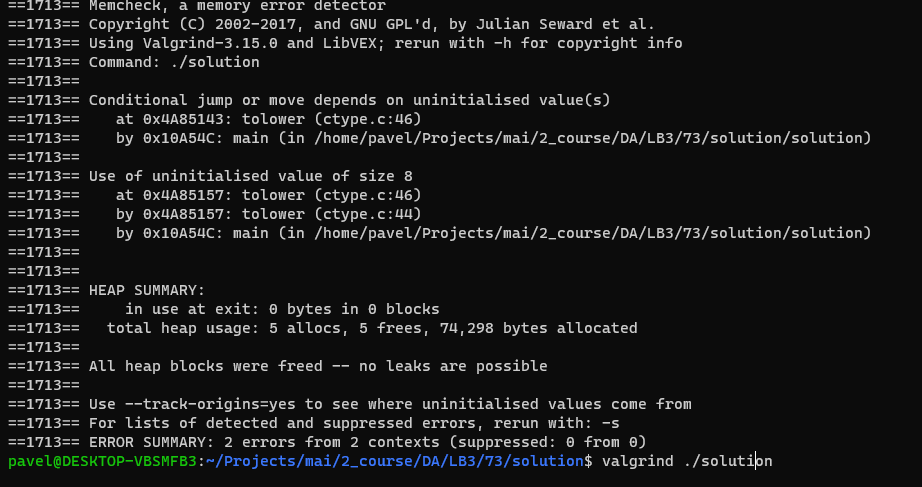
\includegraphics[width=\linewidth]{img_1.png}

Источником этой проблемы стала попытка приведения строки к ничжнему регистру вне зависимости была ли она введена. То есть мы пыталить изменить не инициализированную область памяти.

Листинг неисправного кода:
\begin{lstlisting}[language=C++]
friend std::istream& operator>>(std::istream &in, TString &str)
{
	
	in >> str.str;
	str.lower();

	while(str.str[str.size] != '\0')
		++str.size;
	return in;
}
\end{lstlisting}

Исправить это можно сделав ввод условием при котором выполняется оставшаяся часть.

Исправленный вариант:
\begin{lstlisting}[language=C++]
friend std::istream& operator>>(std::istream &in, TString &str)
{
	if(in >> str.str)
	{
		while(str.str[str.size] != '\0')
			++str.size;
	}
	return in;
}
\end{lstlisting}

{\bfseries Ошибка 2:} При вводе большого теста Valgrind выводит большое количество ошибок:

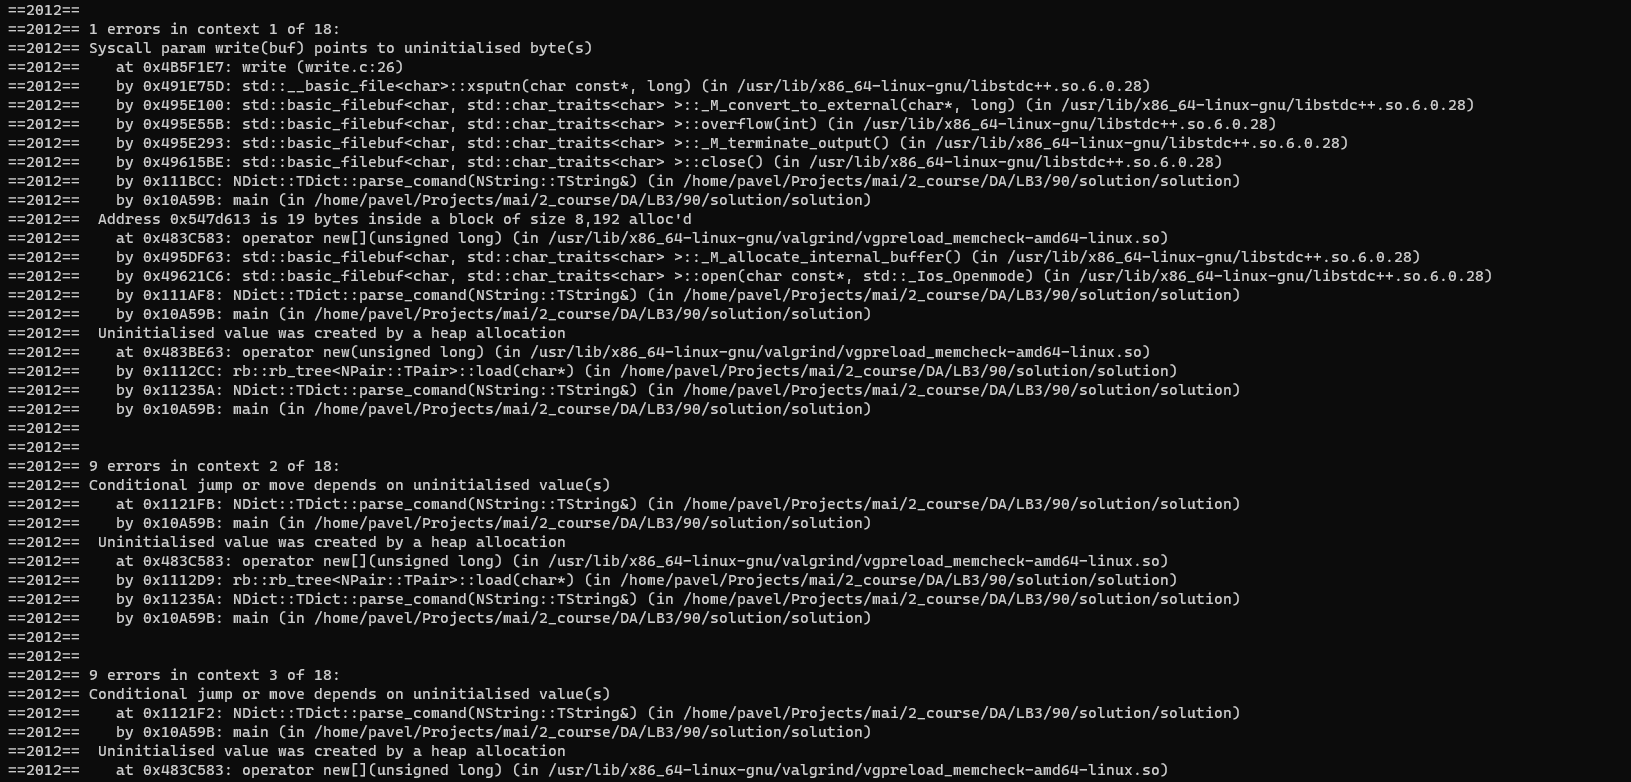
\includegraphics[width=\linewidth]{img_2.png}

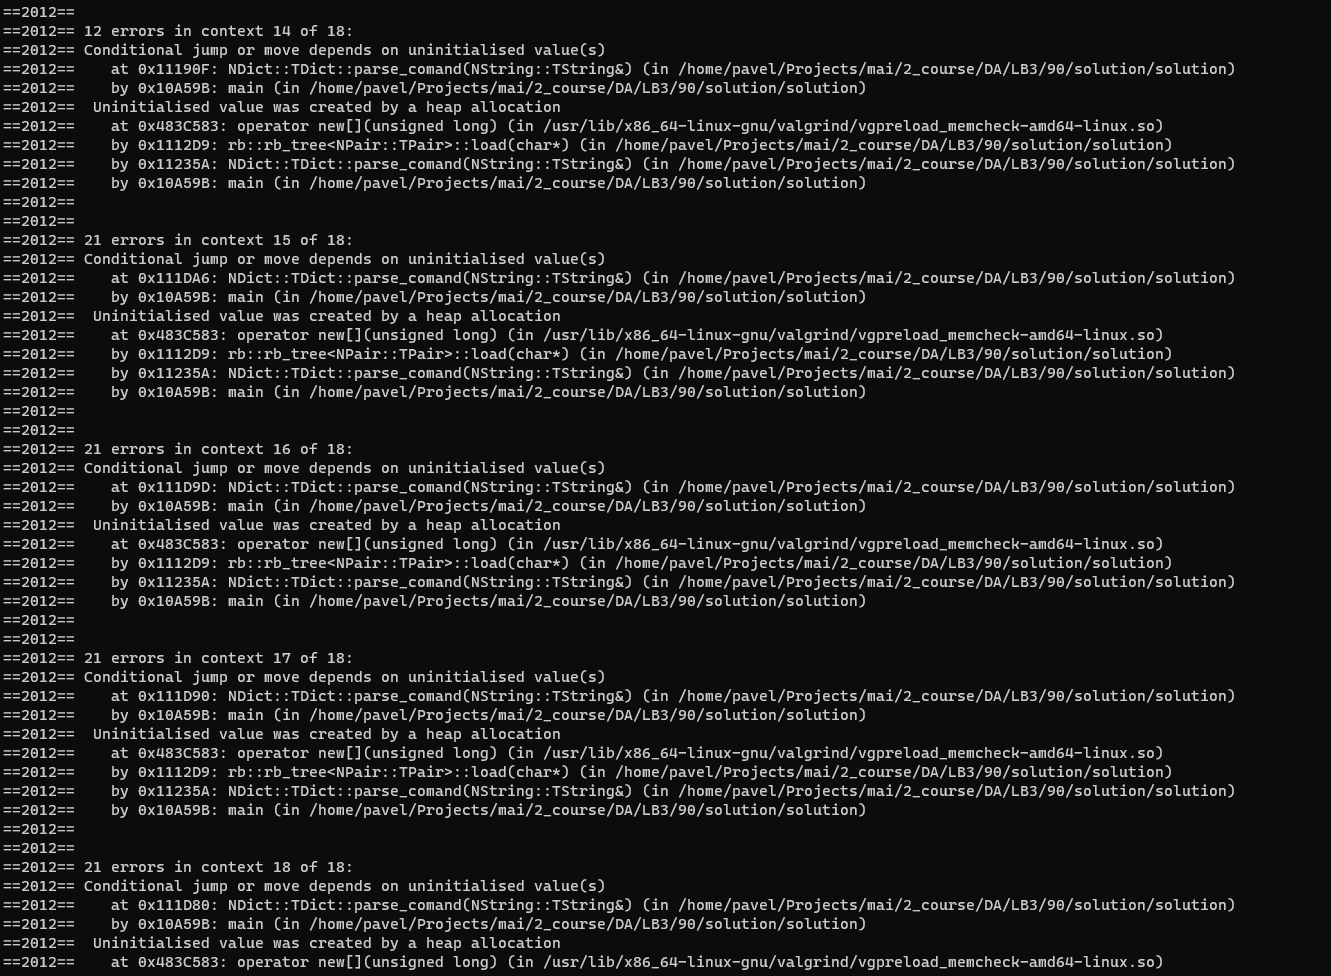
\includegraphics[width=\linewidth]{img_3.png}

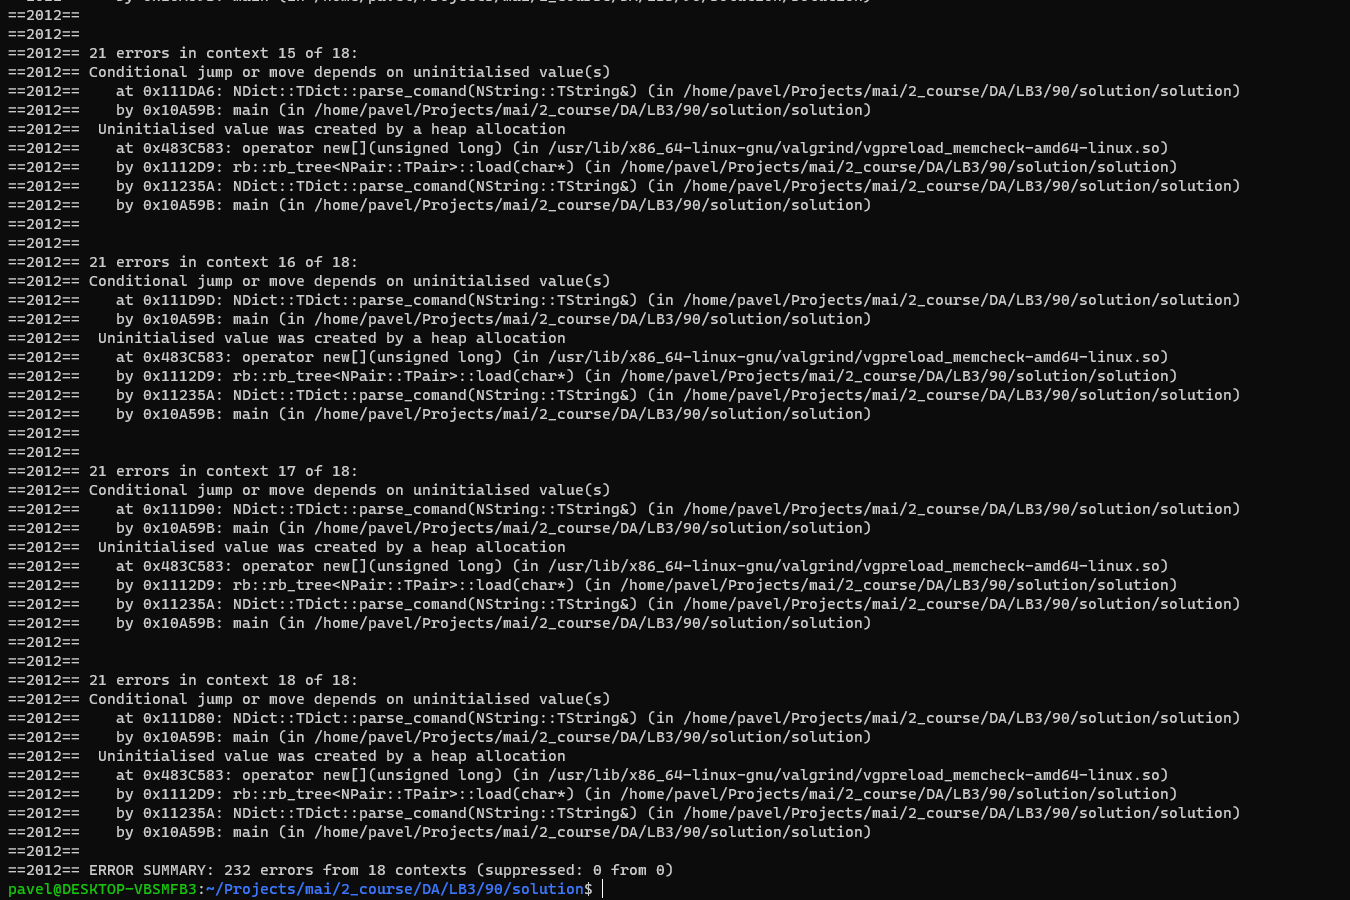
\includegraphics[width=\linewidth]{img_4.png}

При тестировании я пришел к выводу, что эти ошибки появляются после загрузки пустого файла, поэтому следует искать ошибку там. Ошибка оказалась в условии. При прочтеннии пустого файла не начиналось чтение из файла, но при этом создавался "мусорый" элемент. Поэтому решением будет поместить код отвечающий за создание элемента под тоже условие.

Листинг неисправного кода:
\begin{lstlisting}[language=C++]
Root = new rb_tree_elem<T>;
Root->Par = Nil;
Root->Left = Nil;
Root->Right = Nil;
if(!isFileEmpty(ch))
load_tree(Root,rf);
\end{lstlisting}

Исправленный вариант:
\begin{lstlisting}[language=C++]
Root = Nil;
if(!isFileEmpty(ch)){
	Root = new rb_tree_elem<T>;
	Root->Par = Nil;
	Root->Left = Nil;
	Root->Right = Nil;
	load_tree(Root,rf);
}
\end{lstlisting}

После исправления этих ошибок мы получаем полностью рабочаю программу.

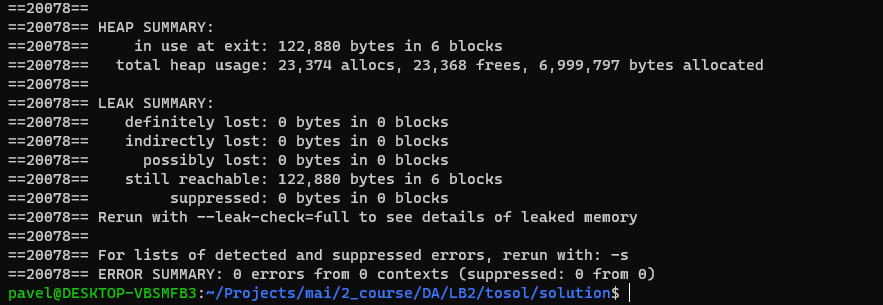
\includegraphics[width=\linewidth]{img_5.png}

После этого можно перейти к профилированию.

Callgrind - одна из самых удобных утилит для анализа времени исполнения программы. Callgrind выдает отчет в текстовом формате, который удобно просматривать с помощью утилит kcachegrind и qcachegrind, и их помощью можно легко просмотреть колличество вызовов и затратность по времени тех или иных функций.

Создадим отчет Callgrind:

\begin{alltt}
pavel@DESKTOP-VBSMFB3:~/Projects/mai/2_course/DA/LB2$ cat test | valgrind --tool=callgrind ./solution
\end{alltt}

Откроем сгенерированный файл в qcachegrind:

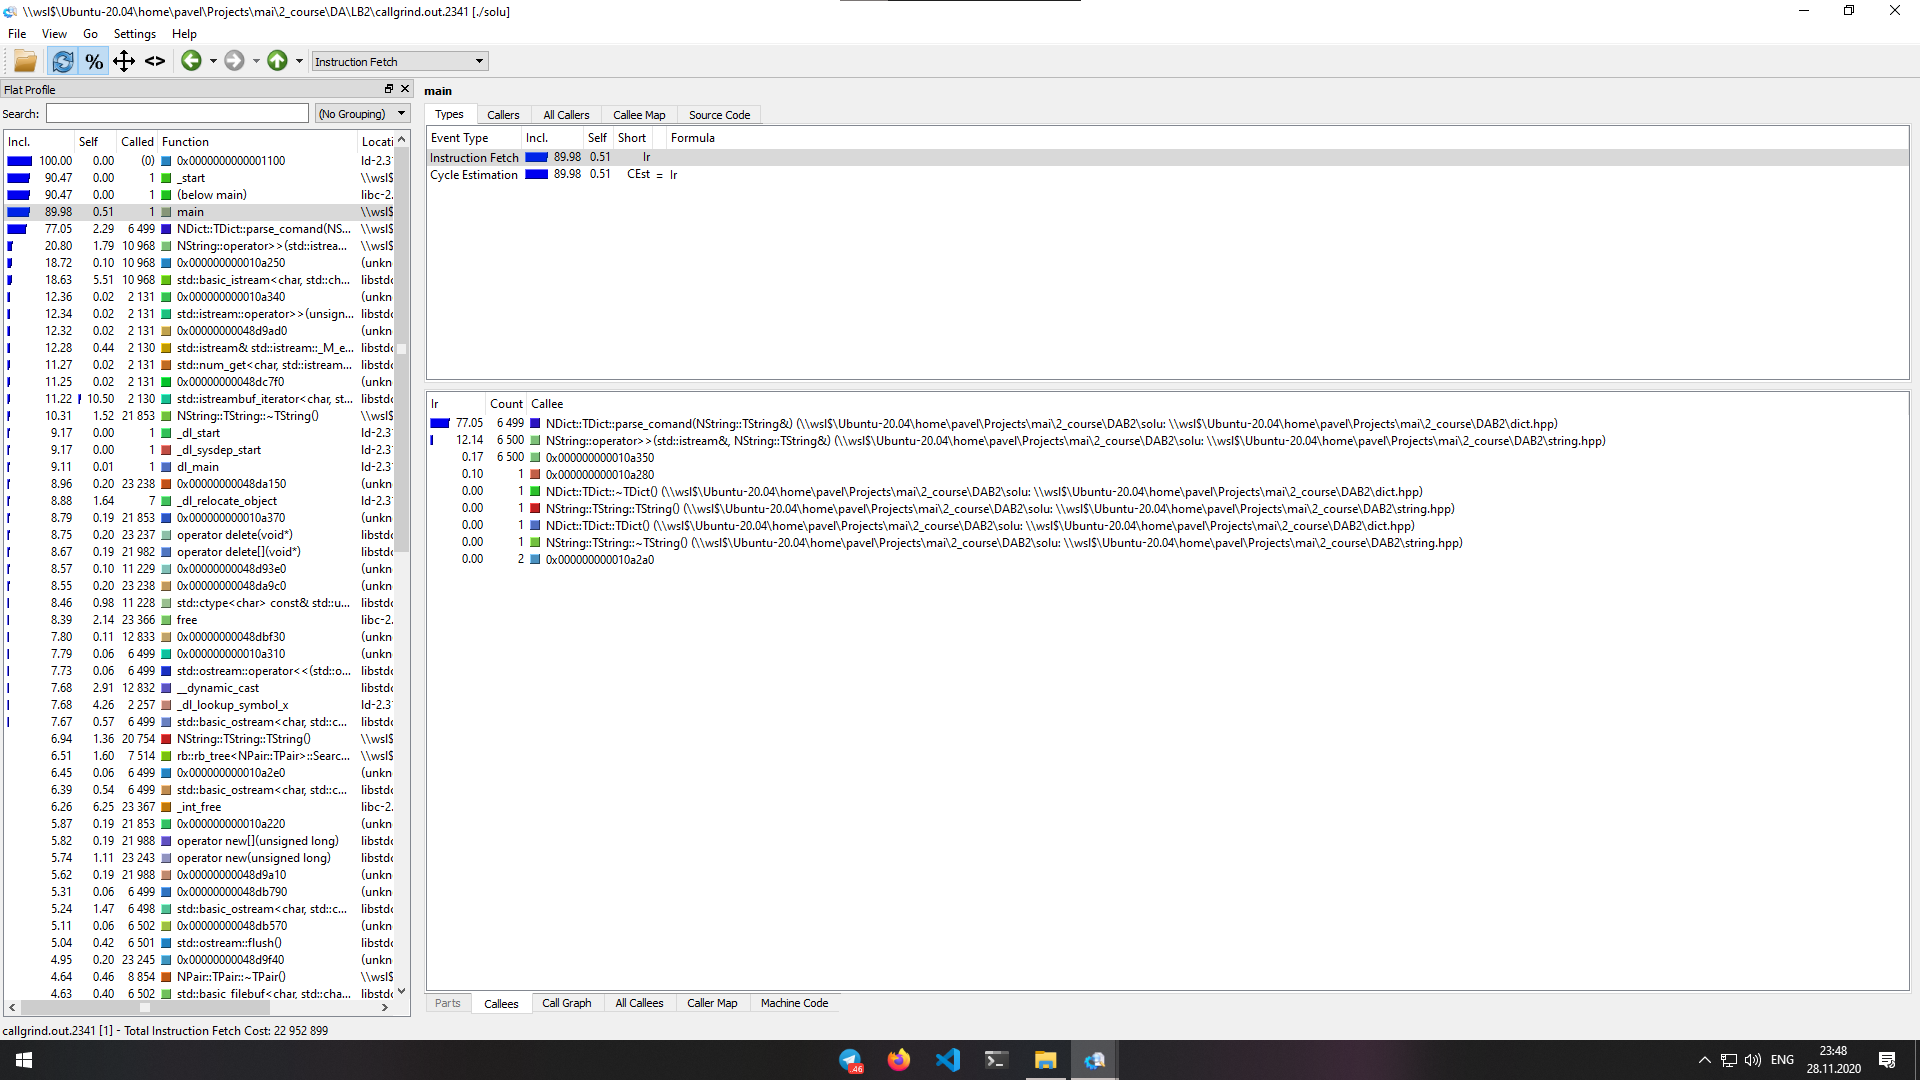
\includegraphics[width=\linewidth]{img_6.png}

Слева мы видим список функций, который мы можем отсортировать по количеству вызовов и времени исполнения, тем самым определяя проблемные участки. Справа сверху можно просмотреть исходный код функции, а снизу например древо вызовов функций. В моем случае я не могу просмотреть код функций, так как код отчета локально обращается к файлам с исходным кодом, из-за этого после перемещения отчета мы не можем обратиться к ним.
\pagebreak

